\chapter{Feature Extraction and Fall Detection}



This chapter covers the 20-dimensional feature vector extracted on the edge device, the cloud inference infrastructure, the rule-based \textit{StreamingFallDetector}, and the real-time React dashboard.

\section{Feature Extraction}

Before transmission to the cloud, the Raspberry Pi extracts a compact 20-dimensional feature vector from each fused radar frame. Points with SNR below 10 dB are discarded. The frame rate is approximately 18 FPS (55 ms inter-frame interval), enabling finite-difference velocity and acceleration estimates. Table 5.1 describes all 20 features.

The three most discriminative features are: (i) $\bar{z}$, which drops rapidly from $\approx$1.0 m (standing) to $\approx$0.2 m (lying) during a fall; (ii) $\Delta z$, which collapses from $\approx$1.6 m (standing) to $\approx$0.3 m (lying); and (iii) $n_{\text{pts}}$, which decreases as the body transitions to a horizontal posture presenting a smaller radar cross-section.

Approximately 36--40 feature vectors are batched into a single JSON file written to a local watch directory. The file watcher then transmits the full batch to the cloud in a single HTTP round trip.


\begin{table}[H]
\caption{20-Dimensional Feature Vector Extracted per Radar Frame}
\label{tab:summary_4}
\centering
\begin{tabularx}{\textwidth}{@{} l X X X @{}}
\toprule
\textbf{Idx} & \textbf{Feature} & \textbf{Source} & \textbf{Description} \\ \midrule
0--2 & $x, y, z$ & Point Cloud & Mean position of all reflections \\
3--5 & $v_x, v_y, v_z$ & Point Cloud & Mean Doppler velocity components \\
6--8 & $a_x, a_y, a_z$ & Computed & Acceleration ($\Delta v / \Delta t$) \\
9 & $n_{\text{pts}}$ & Point Cloud & Number of reflection points \\
10 & $\sigma_{xy}$ & Point Cloud & Horizontal spread: $\text{var}(x) + \text{var}(y)$ \\
11 & $\Delta z$ & Point Cloud & Height range $\max(z) - \min(z)$; body posture indicator \\
12--17 & Track features & Track Data & Position and velocity of primary track \\
18 & $h_{\text{person}}$ & Height Data & Estimated person height (TI algorithm) \\
19 & $h_{\text{bottom}}$ & Height Data & Bottom of bounding box height \\ \bottomrule
\end{tabularx}
\end{table}




\section{Cloud Inference Infrastructure}

The batch JSON file is detected via Linux inotify with sub-millisecond notification latency. A stability check polls file size until stable, ensuring complete JSON write before parsing. The batch is POSTed to the \texttt{/frames/batch} endpoint on AWS EC2 (region \texttt{ap-south-1}, Mumbai), hosted in a Dockerized FastAPI application served by Uvicorn behind Nginx. Table 5.2 summarizes the API fields.

\begin{table}[H]
\caption{Key Fields of the \texttt{/frames/batch} API Endpoint}
\label{tab:summary_5}
\centering
\begin{tabularx}{\textwidth}{@{} l X X @{}}
\toprule
\textbf{Field} & \textbf{Direction} & \textbf{Description} \\ \midrule
\texttt{device\_id} & Request & Unique sensor node identifier \\
\texttt{features} & Request & 20-D float vector for the frame \\
\texttt{timestamp} & Request & ISO 8601 UTC wall-clock time \\
\texttt{human\_count} & Request & Number of tracked persons \\
\texttt{class\_name} & Response & \texttt{"FALL"} or \texttt{"NO-FALL"} \\
\texttt{confidence} & Response & Fraction of tests passed (0.33, 0.67, or 1.0) \\
\texttt{is\_fall} & Response & Boolean fall indicator \\
\texttt{z\_mean} & Response & Centroid height echoed for dashboard display \\ \bottomrule
\end{tabularx}
\end{table}



Per-frame HTTP calls would incur 36 round trips at $\approx$130 ms each, totalling 4.7 s per file---incompatible with real-time operation. Batching into a single POST reduces round-trip overhead to $\approx$150 ms per file.


\section{Rule-Based Fall Detection: \textit{StreamingFallDetector}}

\subsection{Design Rationale}

Fall detection in this system is implemented as a fully deterministic, rule-based classifier called the \textit{StreamingFallDetector}. The decision to implement fall detection using explicit physical rules rather than a learned model was made for five specific reasons:

\begin{itemize}
    \item \textbf{Zero training data requirement:} Immediate deployment without any labelled dataset.
    \item \textbf{Full interpretability:} Each decision directly traceable to specific physical measurements.
    \item \textbf{Sub-millisecond inference time:} Three simple threshold comparisons, orders of magnitude faster than any neural network.
    \item \textbf{CPU-only deployment:} No GPU required on the EC2 instance.
    \item \textbf{Physical grounding:} Thresholds derived directly from biomechanics of human falls, generalizing across subjects without retraining.
\end{itemize}

The \textit{StreamingFallDetector} maintains a rolling window of $N_{\text{win}} = 20$ most recent $\bar{z}$ values, establishing a dynamic baseline of the subject's centroid height that automatically adapts to individual height differences.

\subsection{Three-Test Majority Vote}

Each incoming frame is evaluated against three independent physical tests, as summarized in Table 5.3. A fall event is declared when at least two of the three tests pass simultaneously.

The confidence score is computed as $C = N_{\text{pass}} / 3$, yielding values of 0.33, 0.67, or 1.0. After a fall is declared, a 30-frame ($\approx$1.65 s) suppression cooldown prevents repeated triggers from the same event. The first $N_{\text{win}} = 20$ frames are treated as a warm-up period during which the $\bar{z}$ baseline is established. Figure 5.1 illustrates the per-frame decision flow.

\begin{figure}[htbp]
    \centering
    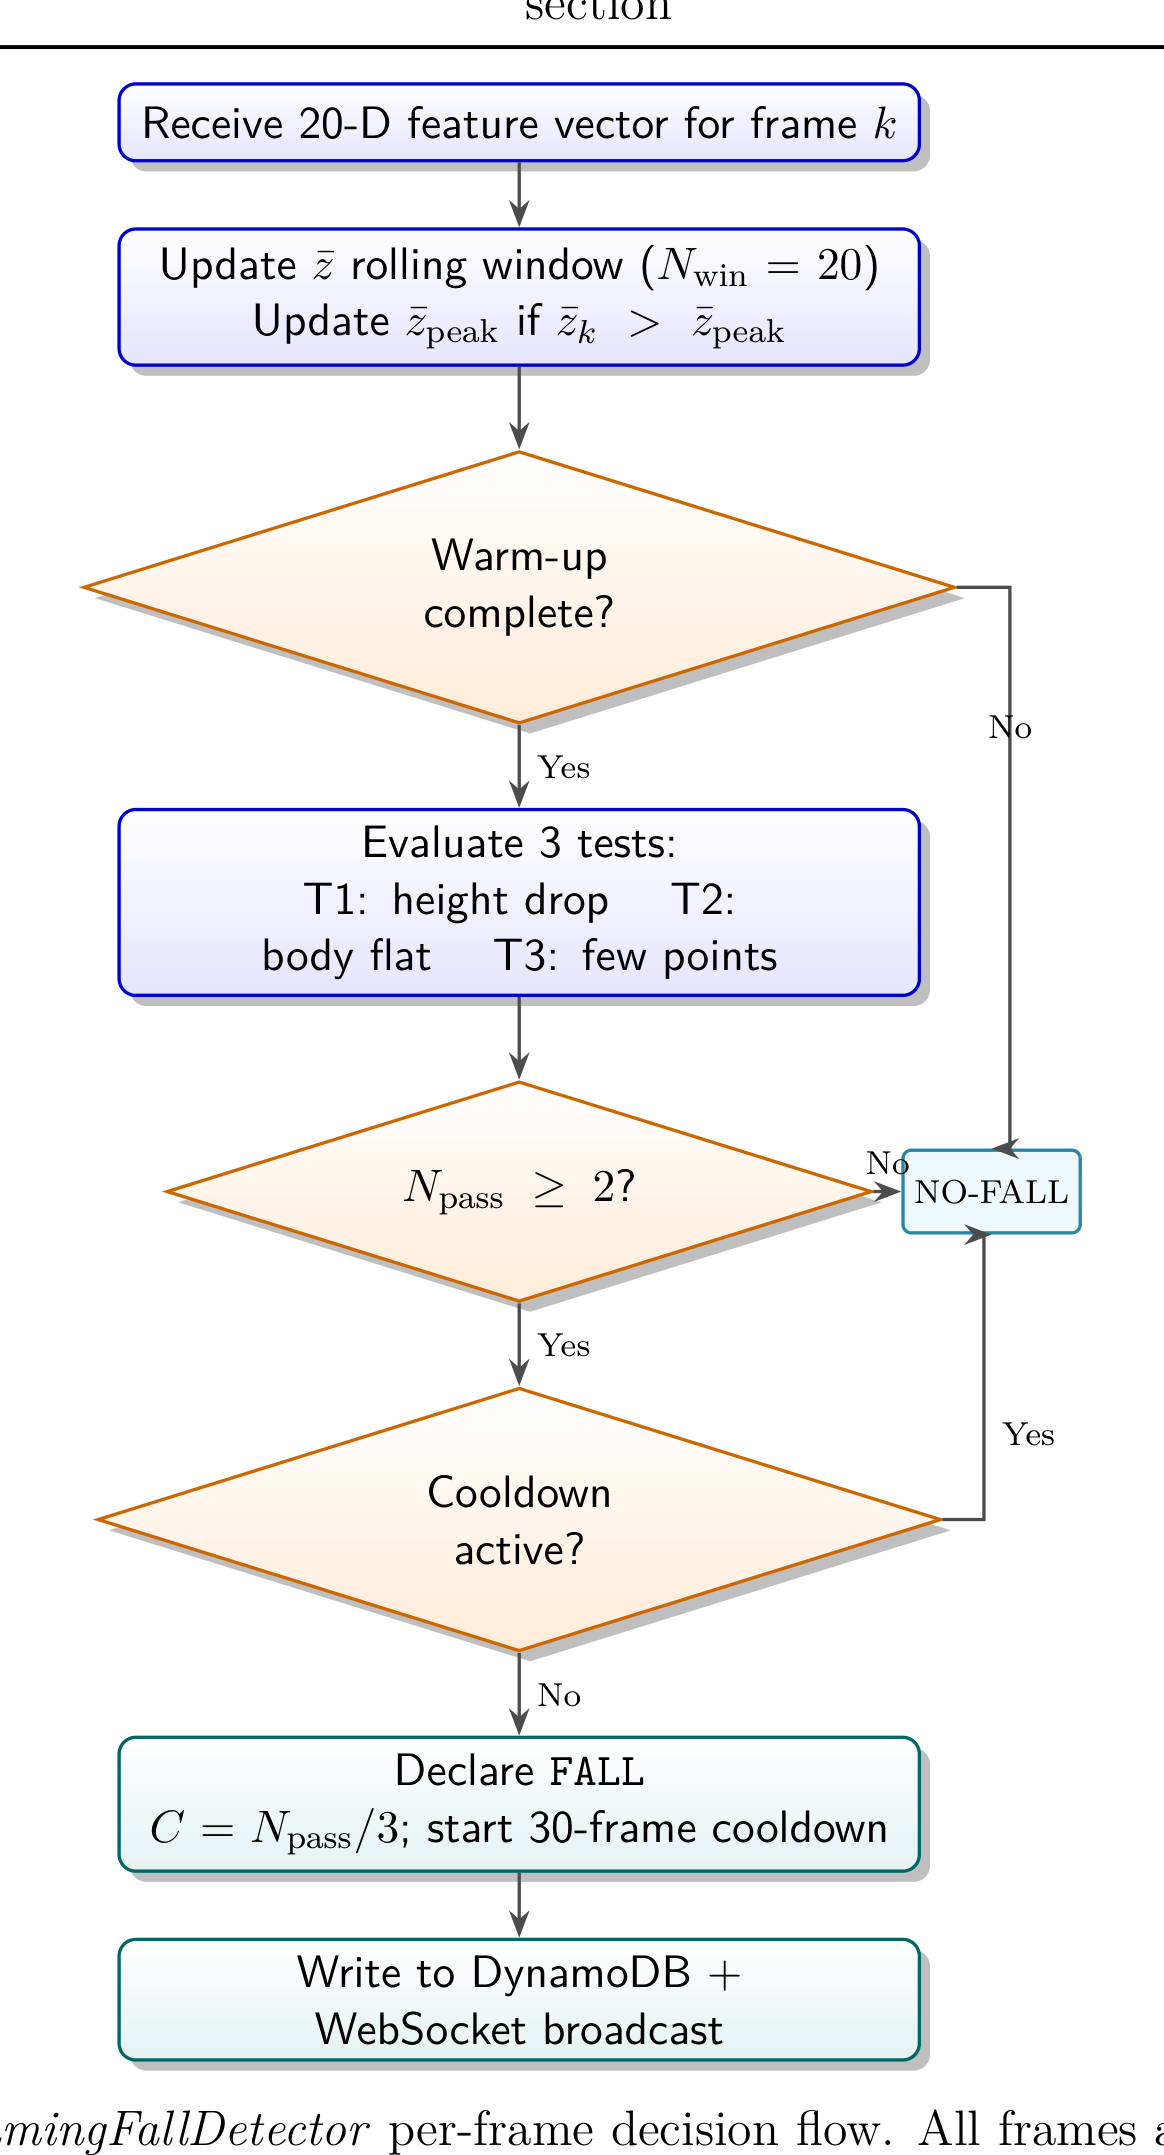
\includegraphics[width=\textwidth,height=0.8\textheight,keepaspectratio]{Figures/flowchart_p24.png}
    \caption{\textit{StreamingFallDetector} per-frame decision flow}
    \label{fig:decision_flow}
\end{figure}


\begin{table}[H]
\caption{\textit{StreamingFallDetector} Three-Test Majority Vote Criteria}
\label{tab:summary_6}
\centering
\begin{tabularx}{\textwidth}{@{} l X X @{}}
\toprule
\textbf{Test} & \textbf{Condition} & \textbf{Physical Rationale} \\ \midrule
Height drop & $z_{\text{peak}} - z_{\text{current}} \geq 0.50$ m & Person's centroid drops significantly below recent maximum \\
Body flat & $\Delta z \leq 0.50$ m & Vertical extent of point cloud collapses; body is horizontal \\
Few points & $n_{\text{pts}} \leq 8$ & Lying body presents a smaller radar cross-section \\ \bottomrule
\end{tabularx}
\end{table}



\subsection{Persistence and Real-Time Broadcast}

All inference results are broadcast immediately via WebSocket to every connected dashboard client with EC2-to-browser latency below 50 ms. Only confirmed FALL events are persisted to AWS DynamoDB (\texttt{radar\_events} table, partition key \texttt{device\_id}, sort key \texttt{ts}) with a 24-hour TTL. The \texttt{/history} REST endpoint supports querying recent fall events for dashboard pre-population on page load.

\section{Heterogeneous Fusion Results}

Figure 5.2 visually validates the advantages of heterogeneous radar fusion by comparing a top-down snapshot of a single-person target across three configurations: IWR6843 only, AWR1843 only, and the fused output. The data represents a real-world scenario where the two disparate sensors are deployed with a spatial and angular offset.

\begin{figure}[H]
    \centering
    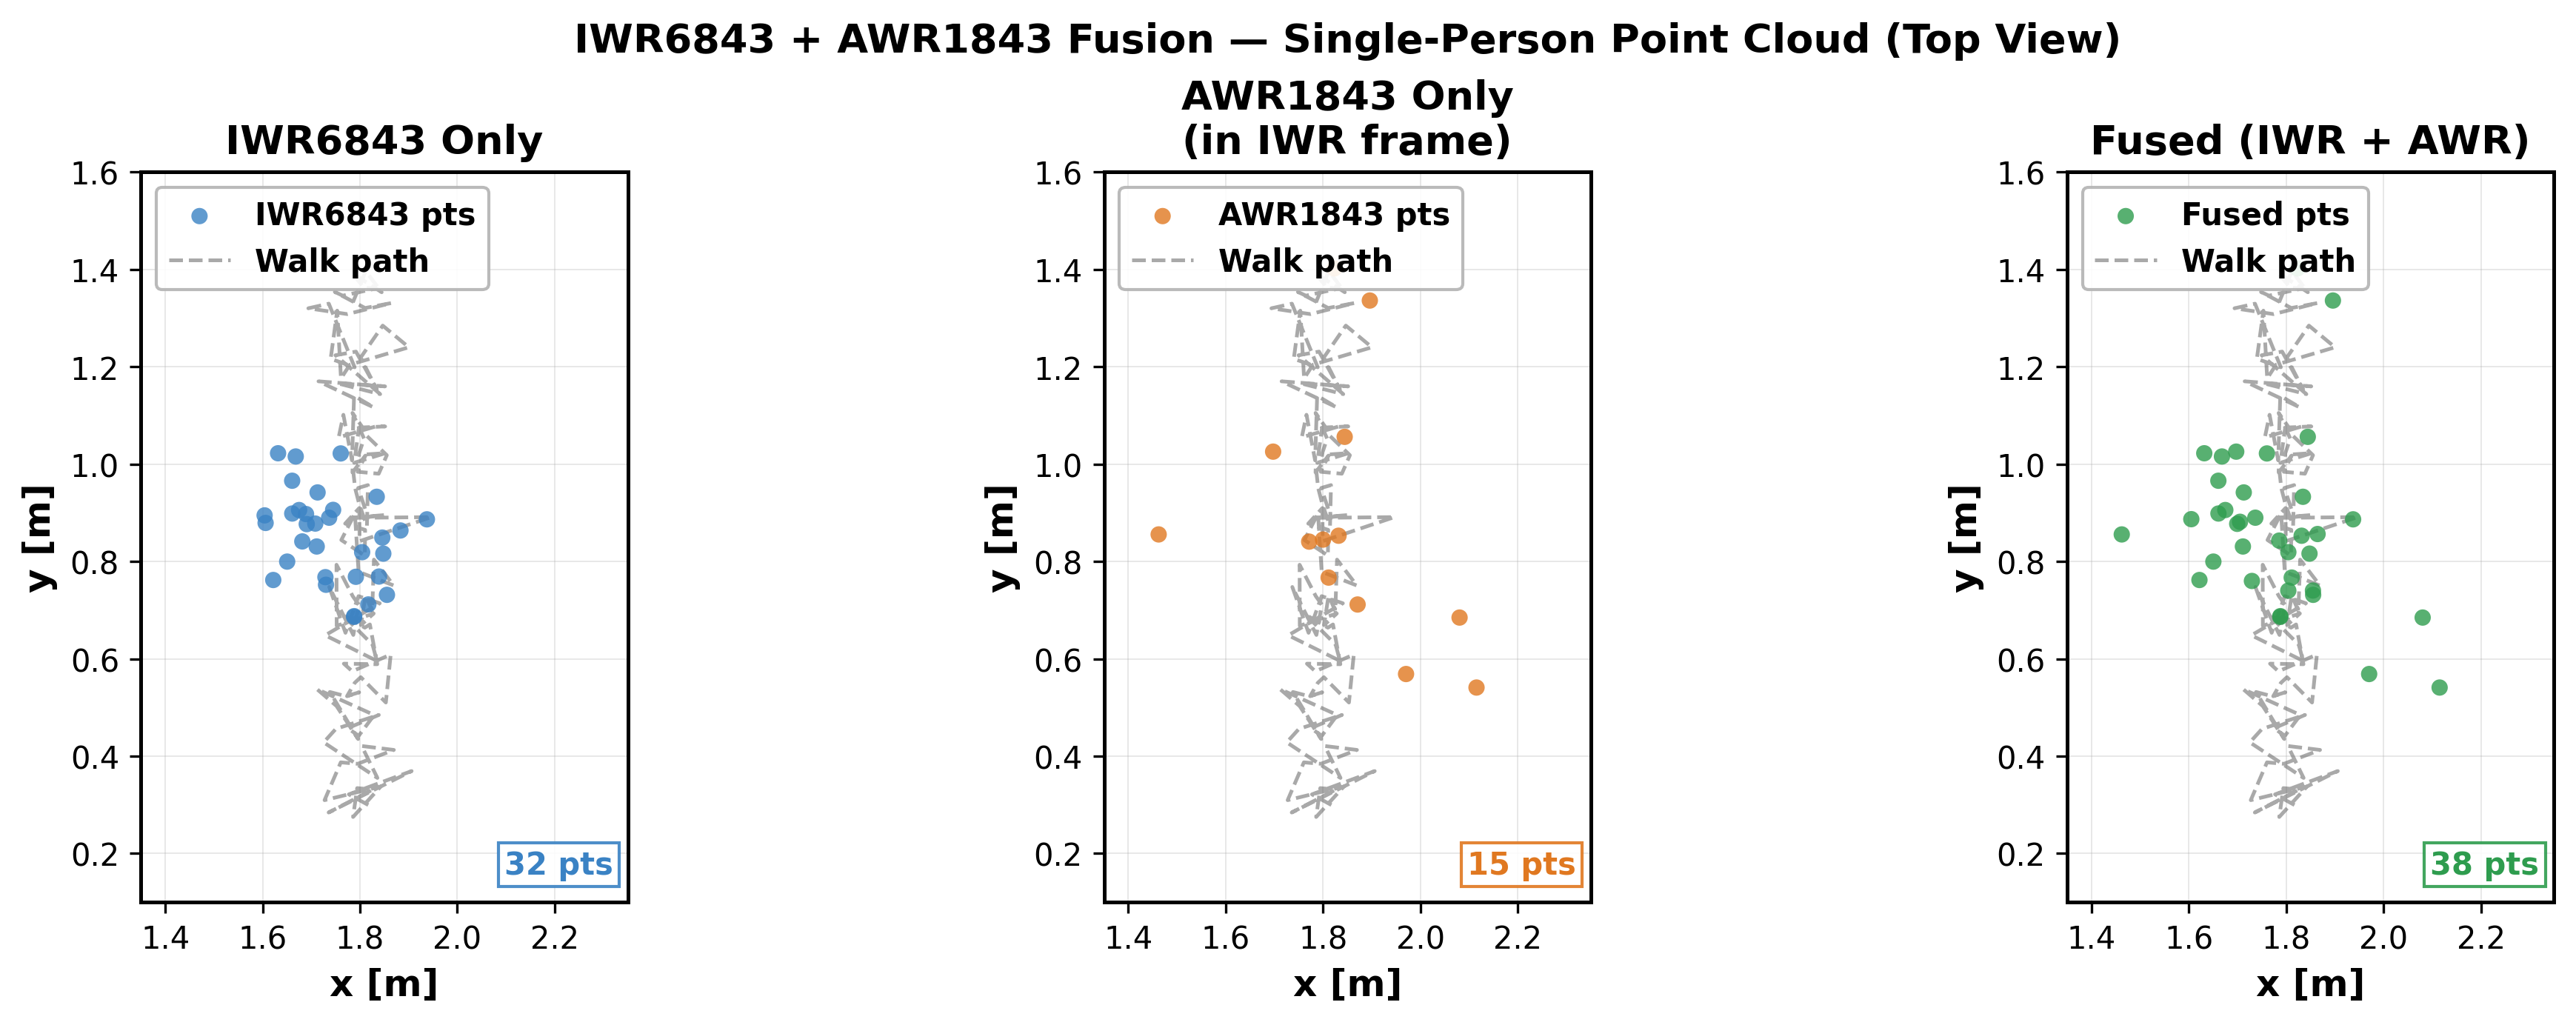
\includegraphics[width=\textwidth]{Figures/fig9_iwr_awr_fusion.png}
    \caption{Single-Person Point Cloud Validation: IWR6843 vs. AWR1843 vs. Fused Output}
    \label{fig:iwr_awr_fusion}
\end{figure}

\textbf{Key Observations from Figure 5.2:}
\begin{itemize}
    \item \textbf{Sensor-Specific Characteristics:} The left panel illustrates the IWR6843's high angular resolution, producing a dense, tightly clustered point cloud (32 points) that tracks the true target path closely. The middle panel shows the AWR1843 data mathematically transformed into the IWR coordinate frame; its detections are sparser (15 points) and exhibit a wider spatial spread due to differing antenna profiles and SNR characteristics.
    \item \textbf{Fusion Enhancement:} The right panel demonstrates the efficacy of the proposed spatial alignment and voxel downsampling pipeline. By successfully transforming and merging the heterogeneous data streams, the fused point cloud achieves a higher point density (38 points) than either individual sensor.
    \item \textbf{Conclusion:} The fused output leverages the high resolution of the IWR while incorporating the supplemental spatial awareness of the AWR, resulting in a richer, more robust target representation without succumbing to the increased noise floor of the automotive sensor.
\end{itemize}

\section{Real-Time Dashboard}

The React dashboard is served from AWS S3 static hosting and connects to the WebSocket endpoint at page load. It maintains a rolling buffer of 200 recent inference events and pre-populates history via a \texttt{GET /history} request on initialization. The layout comprises a current-activity panel showing class label, confidence, centroid height, height range, point count, and human count, alongside a scrollable inference history. Upon a confirmed fall detection, the dashboard switches to a prominent visual alert state.

Figure 5.3 shows the real-time dashboard in its normal operating state.

\begin{figure}[H]
    \centering
    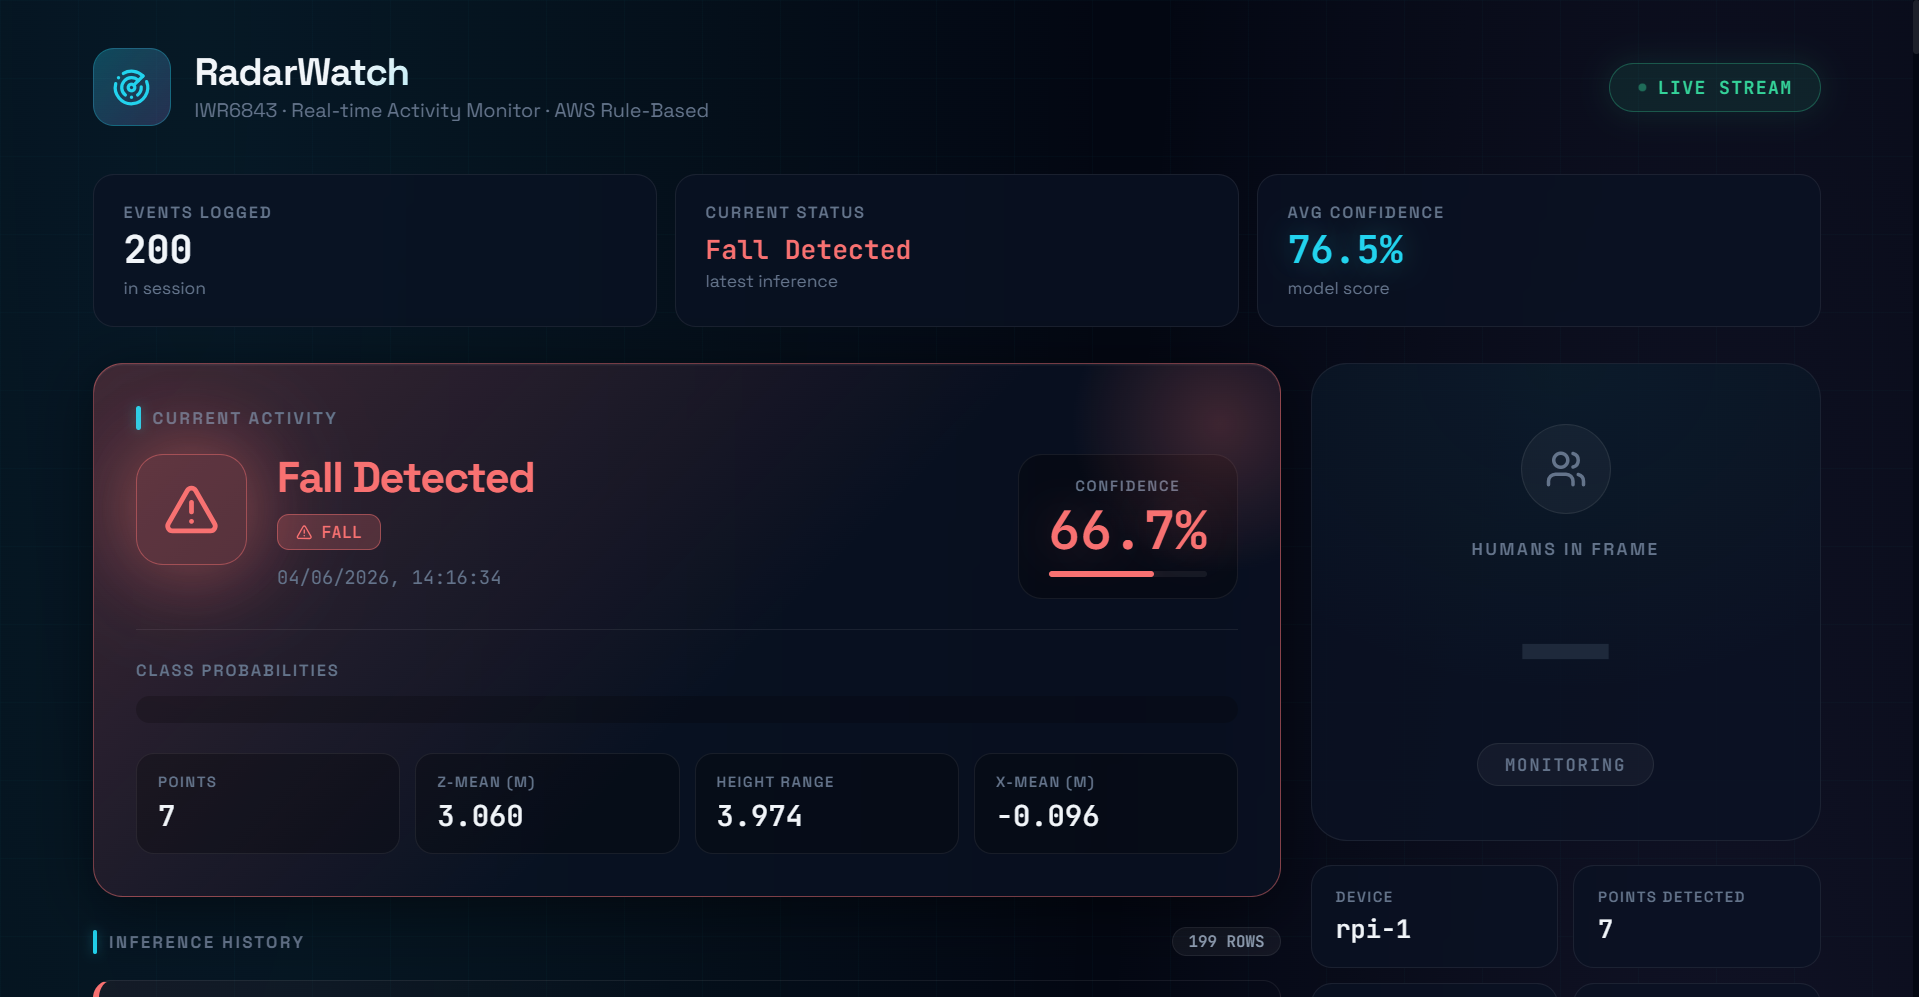
\includegraphics[width=\textwidth]{Figures/fig3_dashboard1.png}
    \caption{Real-Time Activity Dashboard}
    \label{fig:dashboard}
\end{figure}
